% Curator prediction mismatch — one-pager.
% Structure: Research question / Context / Methods / Figure / Takeaways.
% Compile: `make` (pdflatex via latexmk).

\documentclass[10pt]{article}

\usepackage[margin=0.9in]{geometry}
\usepackage{graphicx}
\usepackage{enumitem}
\usepackage{caption}
\usepackage[hidelinks]{hyperref}
\usepackage{parskip}

\setlist[itemize]{leftmargin=1.2em,topsep=0.2em,itemsep=0.15em,parsep=0pt}

\pagestyle{empty}

\begin{document}

% ----- Title block (centered, preprint style) -----
\begin{center}
{\Large\bfseries An LLM's hypothesized task difficulties don't predict another LLM's empirical difficulty\par}
\end{center}
\vspace{0.2em}
\hrule
\vspace{0.4em}
\begin{center}
Tyler Lifke\\[0.15em]
{\small 2026-05-12 \,\textbullet\, \href{https://github.com/tlifke/morel-research}{tlifke/morel-research} \,\textbullet\, Study 001: Investigation 006}
\end{center}
\vspace{0.2em}
\hrule
\vspace{0.8em}

\section*{Research question}
PROSE GOES HERE.

\section*{Context}
PROSE GOES HERE.

\section*{Methods}
PROSE GOES HERE.

\begin{figure}[h]
  \centering
  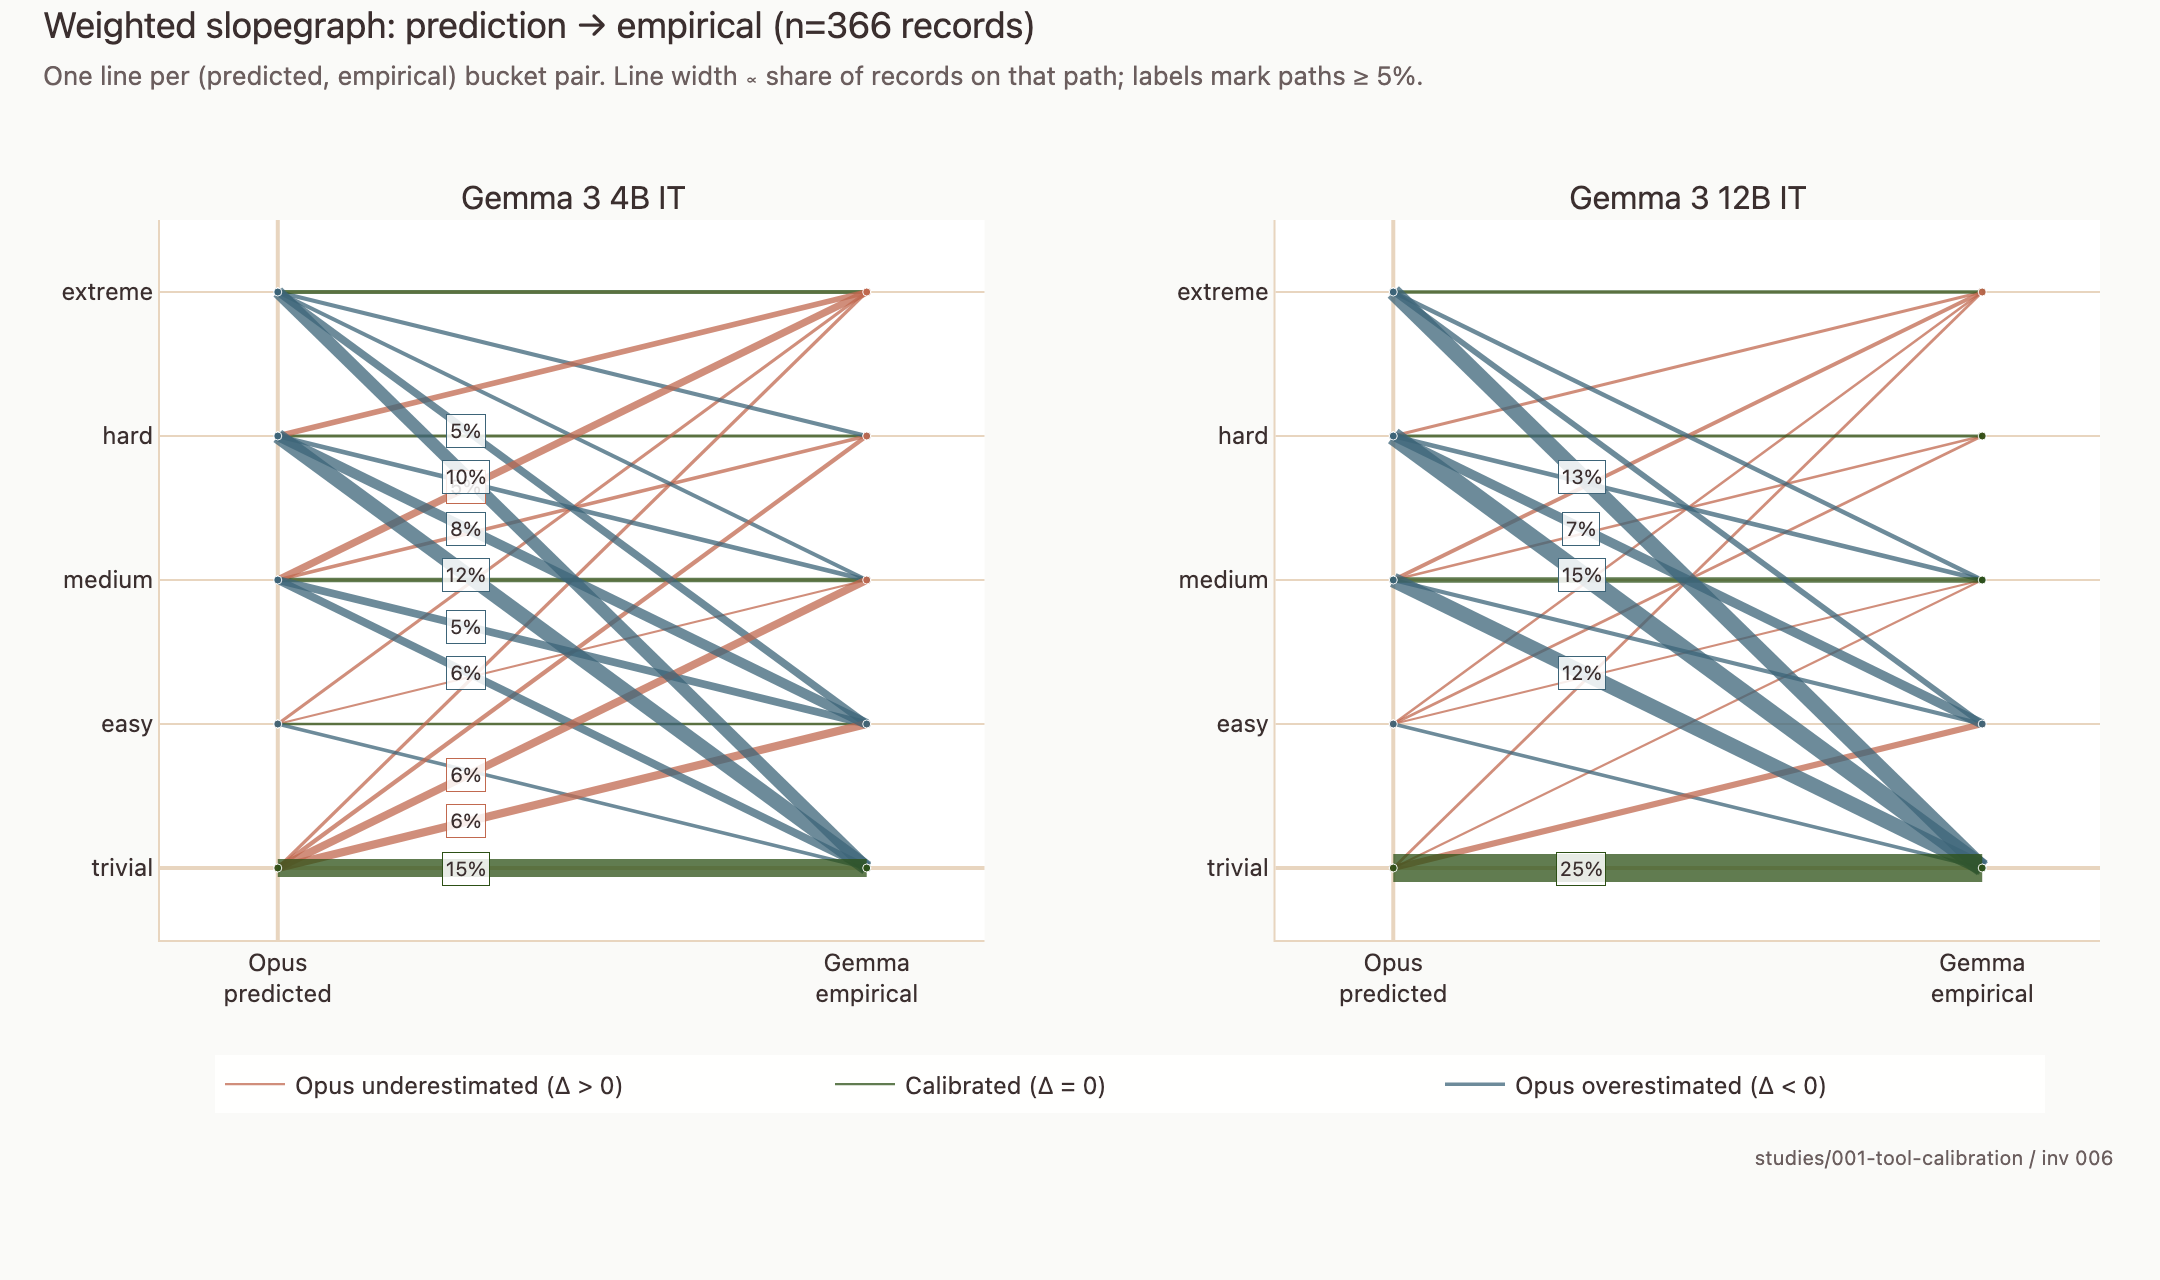
\includegraphics[width=0.95\linewidth]{../../../investigations/006-temperature-prompt/figures/a3_bulk/prediction_slopegraph_weighted.png}
  \caption{ONE-SENTENCE CAPTION THAT SAYS WHAT TO SEE.}
\end{figure}

\section*{Takeaways}
\begin{itemize}
  \item TAKEAWAY TIED TO THE FIGURE.
  \item TAKEAWAY ON A KEY LIMITATION.
  \item OPTIONAL: ADDITIONAL RESULT THAT DIDN'T MAKE THE FIGURE.
  \item OPTIONAL: ADDITIONAL TAKEAWAY (3--5 total).
\end{itemize}

\end{document}
